\section{Requirements}
\label{sec:Requirements}



%openCV, bmob
\subsection{Overview} 
\label{RequirementsOverview}
\paragraph{}
The Gift Box Project was conceived by Dr. Hunt inspired by the very popular game Pokemon Go. For this project, Dr. Hunt served as the supervisor and the sponsor.
\par The supervisor met with the developer several times to gather informal functional requirements of this program. These informal functional requirements helped to define the scope of the program as well as capture the true nature and purpose of the application. During the first of these informal meetings, the supervisor provided samples of the processed pictures with a wall-hanging and identified how to select a region. Based on the information collected from these meetings, the requirement document version 1.0 was created, in which the following requirements were listed:
\begin{itemize}
\item This project will support both a web interface and an Android application.
\item The gifts sent by a user can be selected from a pre-defined library or created by users. 
\item The gift will be projected onto the region chosen by user.
\item GPS navigation allows users to find gifts but it only supports 2D locations. 
\item The application will attempt to robustly allow gifts to be found from a variety of angles, distances, and lighting conditions.
\end{itemize}
\par The project initially included the development of the image comparator which include image recognition and image transformation algorithms. However, the scope of the image comparator was too large and imposed too much complexity on the developer. To address this complexity, the developer, with assistance from Dr. Hunt, decided to use third-party software packages which would be able to perform the functionalities of image recognition. A software package was chosen depending on the required features. The scope of the program was therefore appropriately reduced by using the third-party software for the complex image recognition.
\par The detailed functional requirements are described in Section \ref{FunctionalRequirements} Functional Requirements. 

\subsection{Functional Requirements}
\label{FunctionalRequirements}
\paragraph{}
This program only supports one role, the System User for Android Application. Figure \ref{Use Cases Diagram} gives a Use Case diagram for the System User.
\par As shown in the Figure \ref{Use Cases Diagram}, there are eight use cases in the diagram. Each use case describes a functional requirement. These functional requirements are narrated as follows:

\begin{figure}[htb]
\centering
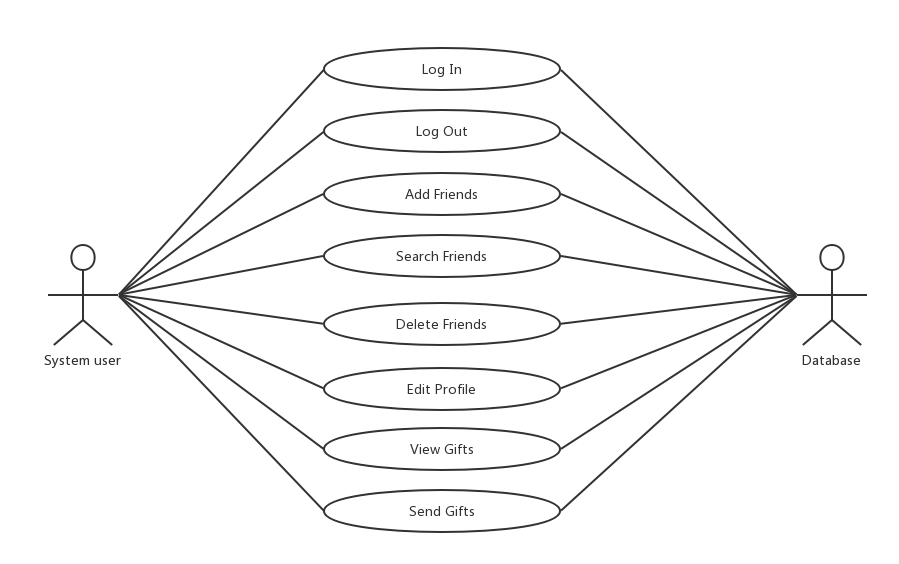
\includegraphics[width=.5\textwidth]{section02/assets/UseCase.png}
\caption[Use Case Diagram for Android Application]{\label{Use Cases Diagram}Use Case Diagram for Android Application}
\end{figure}

\begin{itemize}
\item The \bsq{Log In} function allows users to log in to the system.
\item The \bsq{Log Out} function allows users to log out of the system.
\item The \bsq{Add Friends} function allows users to add other users as friends. This add function doesn't need other users' agreement.
\item The \bsq{Search Friends} function allows users to search other users by username.
\item The \bsq{Delete Friends} function allows users to delete friends from their friends list.
\item The \bsq{Edit Profile} function allows users to edit their password and portrait information. The username and email cannot be changed after registration. 
\item The \bsq{View Gifts} function allows users to view their gifts. Gifts are filtered based on \bsq{Sent} or \bsq{Received}.
\item The \bsq{Send Gifts} function allows users to send virtual gifts to other users.
\end{itemize}
\par The web interface contains the same functionalities as the Android application except for the \bsq{Send Gift} functionality.  Also, the web interface doesn't display those gifts that have not yet been found.
\subsection{Selection of Life Cycle Model}
\paragraph{} At the project inception, we recognized several factors that would affect the development strategy. These factors are listed below.
\begin{itemize}
\item Lack of detailed specification for the GUI.
\item Lack of experience with image recognition.
\item Potential misunderstandings between the project sponsor and the developer.
\end{itemize}
\par To address these factors, we determined to use an adaptive software development model. The adaptive model is a method of software development where the model is designed, implemented and tested incrementally until the product is finished. 
\par Compared to other models, this one will check the consistency between requirements in each iteration. Developers ensure that the product is partially ready with the selected requirements and customers can see the progress of the development process. The graphical illustration of incremental prototyping model is shown in Figure \ref{IncrmentalModel}. In this figure, the `Conventional` line describes the waterfall model where increased functionality generally takes more time to obtain than the incremental approach. The implementation of a new subset of functionalities is obtained quicker in the incremental approach and must be approved by the customer before adding the next subset. This can also be called  the “staircase model”.

\par As a result, each partial functionality can be checked in each interaction and developers will be able to obtain feedback for correcting minor inconsistencies between the delivered product and the user expectations.  Also, if minor alterations to the requirements are indicated, these changes can be addressed within each increment.

\begin{figure}[htb]
\centering
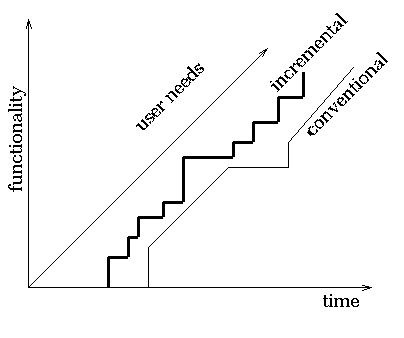
\includegraphics[width=.5\textwidth]{section02/assets/IncrementalModel.png}
\caption[Graphical Illustration of Incremental Prototyping Model]{\label{IncrmentalModel}Graphical Illustration of Incremental Prototyping Model}
\end{figure}

\par Each increment includes the completion of several functional requirements. This project involved seven total increments.  The functional requirements associated with each increment were determined by the sponsor and the developer.  The order in which the requirements for each iteration were determined was dependent upon their general importance and their contribution to the entire system.
\par Functionalities concerning image recognition procedure  and image processing should have a higher priority than others. The increments that occurred in this project are listed below:
\begin{itemize}
\item Increment 1: Graphical User Interface functionalities related to basic user interaction.
\item Increment 2: Image recognition's functionalities related to application interaction.
\item Increment 3: Image perspective functionalities related to application interaction.
\item Increment 4: Enhancing application review and evaluation.
\item Increment 5: System configuration.
\item Increment 6: Writing and executing test cases.
\item Increment 7: Enhancing interactivity of Graphical User Interface.
\end{itemize}